\documentclass{beamer} % "Beamer"Просто текст
\usetheme{Berkeley} % Search online for beamer themes to find your favorite or use the Berkeley theme as in this file.

\usepackage{color} % It may be necessary to set PCTeX or whatever program you are using to output a .pdf instead of a .dvi file in order to see color on your screen.
\usepackage{graphicx} % This package is needed if you wish to include external image files.

\theoremstyle{definition} % See Lesson Three of the LaTeX Manual for more on this kind of "proclamation."
\newtheorem*{dfn}{A Reasonable Definition}               

\title{A Sample Beamer Presentation}
\author{Eric Towne} 
\institute{Bates College}
%\date{January 6, 2012} 
% Remove the % from the previous line and change the date if you want a particular date to be displayed; otherwise, today's date is displayed by default.

\AtBeginSection[]  % The commands within the following {} will be executed at the start of each section.
{
\begin{frame} % Within each "frame" there will be one or more "slides."  
\frametitle{Presentation Outline} % This is the title of the outline.
\tableofcontents[currentsection]  % This will display the table of contents and highlight the current section.
\end{frame}
} % Do not include the preceding set of commands if you prefer not to have a recurring outline displayed during your presentation.

\begin{document}

\begin{frame} 
\titlepage
\end{frame}

\section{What Can Happen at a Critical Point?} % Since this is the start of a new section, our recurring outline will appear here.

\begin{frame} 
\frametitle{The Usual Suspects}

You might think that if $f'(0)=0$ (and $f$ is not a constant function) then at $x=0$, $f$ must have

\begin{itemize}
\pause \item a local maximum, or % Each \pause creates a new slide within the frame.
\pause \item a local minimum, or
\pause \item an inflection point.
\end{itemize}  

\pause If that's what you think, then you are ... \pause (notice that we're giving you time to reconsider!) ... \pause wrong.

\end{frame}

\begin{frame}
\frametitle{A Counterexample}

Consider the function 

$$ f(x)=
\begin{cases} % See Lesson Twelve of the LaTeX Manual for more on cases. 
x^2\sin(1/x), &\text{if }x\neq0 \\
0, &\text{if }x=0
\end{cases}
$$

Let's see what $f'(0)$ is.

\end{frame}

\begin{frame}
\frametitle{Finding $f'(0)$}

By the definition of derivative,
\begin{eqnarray*} % As usual, the asterisk suppresses the numbering of each line in the array.
f'(0)&=&\pause\displaystyle\lim_{h\to 0}\frac{f(0+h)-f(0)}{h}\\
\pause&=&\displaystyle\lim_{h\to 0}\frac{h^2\sin(1/h)-0}{h}\\
\pause&=&\displaystyle\lim_{h\to 0}h\sin(1/h)\\
\end{eqnarray*}

Since $-h\leq h\sin(1/h)\leq h$ \pause and $\displaystyle\lim_{h\to 0}(-h)=\displaystyle\lim_{h\to 0}(h)=0$, \pause the \uncover<7->{Squeeze }Theorem says \pause $f'(0)=0.$
% The command \uncover<m->{STUFF} means that STUFF will appear starting in the mth slide of the frame.
% The command \uncover<m-n>{STUFF} means that STUFF will appear from the mth slide to the nth slide of the frame.
\end{frame}

\begin{frame}
\frametitle{What Really Happens at $x=0$?}
\begin{columns} % This creates a frame with multiple columns.
\begin{column}{0.5\textwidth} % The first column will be 50% as wide as the width of text on the page.
But $f(x)$ oscillates wildly as $x\to 0$, so even though $f'(0)=0$, $f$ has neither max, min, nor inflection point at $x=0$.
\end{column}

\pause

\begin{column}{0.5\textwidth} % Now begins our second column.
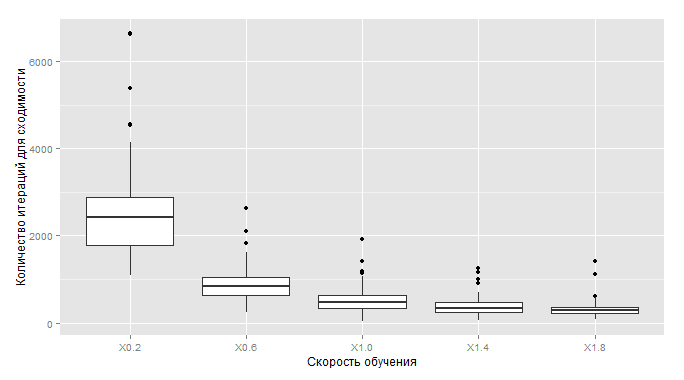
\includegraphics[width=5cm, height=5cm]{graph1.png} % Beamer doesn't like to display .eps files. This .png was converted from .eps using Adobe Acrobat. The file graph1.png should be in the same folder as the .tex file.
\begin{center}
\textcolor{orange}{$y=f(x)$}, \textcolor{red}{$y=x^2$}, \textcolor{green}{$y=-x^2$} % This changes the text color.
\end{center}
\end{column}
\end{columns}
\end{frame}

\section{What Does $g'(c)>0$ Mean?} % Since this is the start of a new section, our recurring outline will appear here.

\begin{frame}
\frametitle{How to Define ``Increasing at a Point''?}
It's natural to think that if $g'(c)>0$ then $g$ must be ``increasing at $x=c$.'' 

\pause But what does ``increasing at $x=c$'' really mean?

\pause \begin{dfn} % We created the proclamation dfn near the start of the document.
A function $g$ is \emph{increasing at $x=c$} if there is an open interval $I=(c-\delta,c+\delta)$ such that \pause if $x_1, x_2\in I$, \pause then $x_1<x_2\Rightarrow \pause g(x_1)<g(x_2)$.
\end{dfn}
\end{frame}

\begin{frame}
\frametitle{Our Function with a Slight Twist}
Let's modify our function to 

$$ g(x)=
\begin{cases}
0.5x+x^2\sin(1/x), &\text{if }x\neq0 \\
0, &\text{if }x=0
\end{cases}
$$

Using the definition of derivative as before, we will find that $g'(0)=0.5$. 
\end{frame}

\begin{frame}
\frametitle{What Really Happens at $x=0$?}
However, $g(x)$ still oscillates enough as $x\to 0$ that there is no open interval containing $x=0$ that satisfies our definition of $g$ increasing at $x=0$ even though $g'(0)>0$.\pause

\begin{center}
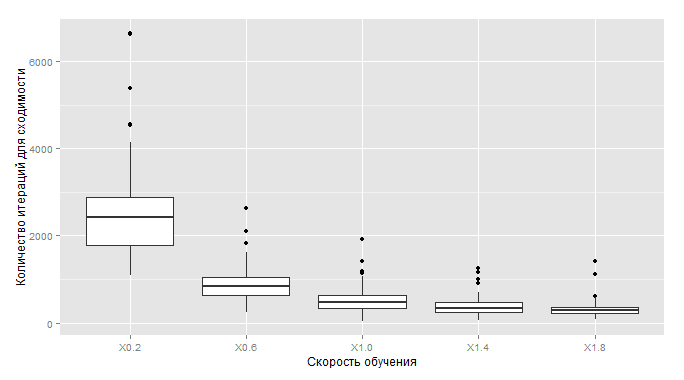
\includegraphics[width=5cm, height=5cm]{graph2.png}

\textcolor{orange}{$y=g(x)$}, \textcolor{red}{$y=x^2+0.5x$}, \textcolor{green}{$y=x^2-0.5x$} 
\end{center}

\end{frame}

\section{Further Work} % Since this is the start of a new section, our recurring outline will appear here.

\begin{frame}
The function $f(x)$ introduced earlier has other interesting properties, one of which is the fact that while $f'(0)$ exists, $f'(x)$ is discontinuous at $x=0$.\vspace{.5cm}

We leave it to you to work this out for yourself and to explore this interesting function further.\vspace{.5cm}

Thank you for your attention today.
\end{frame}

% Some of the ideas for the functions presented in this document came from posts to the ap-calculus group at the Math Forum at http://mathforum.org/kb/forum.jspa?forumID=63.

\end{document}

